% This must be in the first 5 lines to tell arXiv to use pdfLaTeX, which is strongly recommended.
\pdfoutput=1
% In particular, the hyperref package requires pdfLaTeX in order to break URLs across lines.

\documentclass[11pt]{article}

\usepackage[review]{acl}
\usepackage{times}
\usepackage{latexsym}
\usepackage[T1]{fontenc}
\usepackage[utf8]{inputenc}
\usepackage{microtype}
\usepackage{inconsolata}
\usepackage{booktabs}
\usepackage{multirow}
\usepackage{subfiles}
\usepackage{graphicx}
\usepackage{colortbl}

% Commands 
\newcommand{\draftonly}[1]{#1}
\newcommand{\draftcomment}[3]{\draftonly{\textcolor{#2}{[#3]{$_{\textsc{#1}}$}}}}
\newcommand{\lj}[1]{\draftcomment{Lj}{red}{#1}}
\newcommand{\libertus}{\textsc{LiBERTus}}


\title{Team 21a's Submission to the SIGTYP 2024 Shared Task on Word Embedding Evaluation for Ancient and Historical Languages}

\author{Lester James V. Miranda \\
  Allen Institute for Artificial Intelligence \\
  \texttt{ljm@allenai.org} \\
}

\begin{document}

\maketitle

\begin{abstract}
In this paper, we describe Team 21a's submission to the constrained track of the SIGTYP 2024 Shared Task.
Using only the data provided by the organizers, we pretrained a transformer-based multilingual model finetuned on the Universal Dependencies (UD) annotations of a given language.
We also explored the cross-lingual capability of our trained models.
\lj{Our systems achieved}
% TODO: talk about results and scores on the test set
% maybe benchmark against XLM-RoBERTa and mBERT just for a good baseline?
\end{abstract}

\section{Introduction}
This paper describes Team 21a's submission to the \textit{constrained} track of the SIGTYP 2024 Shared Task on Word Embedding Evaluation for Ancient and Historical Languages.
Our general approach involves pretraining a transformer-based multilingual model on the shared task dataset, and then finetuning the pretrained model using the Universal Dependencies (UD) annotations of each language.
Throughout this paper, we will refer to the pretrained model as \libertus{}.
We also explored data sampling and augmentation techniques during the pretraining step to ensure better generalization performance.

Our systems achieved...\lj{stuff}. 
Table \ref{table:main_results} shows our systems' performance on the shared task test set.


We detail our resource creation, model pretraining, and finetuning methodologies.
In addition, we also show the results of our cross-lingual transfer learning setup.

\subfile{tables/main_results.tex}

\section{Methodology}

\subsection{Resource creation}

We constructed the pretraining corpora using the annotated tokens of the shared task dataset.
Then, we explored several data augmentation techniques to ensure that each language is properly represented based on the number of unique tokens.

From our experiments, upsampling underrepresented languages helped reduce our pretraining validation loss.
Figure \ref{fig:unique_tokens} shows that \textsc{latm} has the most number of unique tokens in the corpora.
We upsampled each language by randomly duplicating a document in the training pool until the number of unique tokens is greater than or equal to that of \textsc{latm}.
The same figure also shows the token counts after the augmentation process.

\begin{figure}[t]
\centering
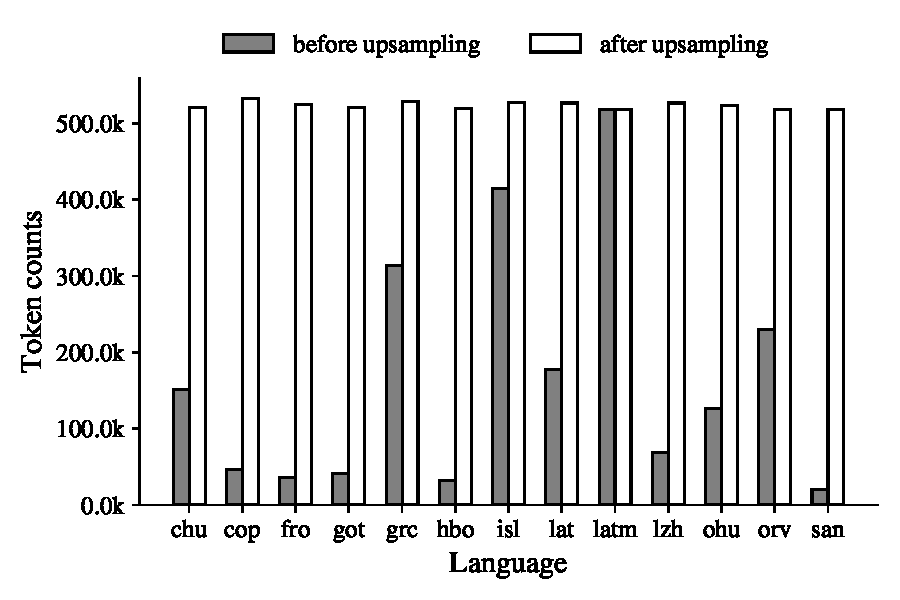
\includegraphics[width=0.5\textwidth]{figures/token_counts.pdf}
\caption{Unique token counts for each language before and after upsampling.}
\label{fig:unique_tokens}
\end{figure}

\subsection{Model Pretraining}

\begin{figure}[t]
\centering
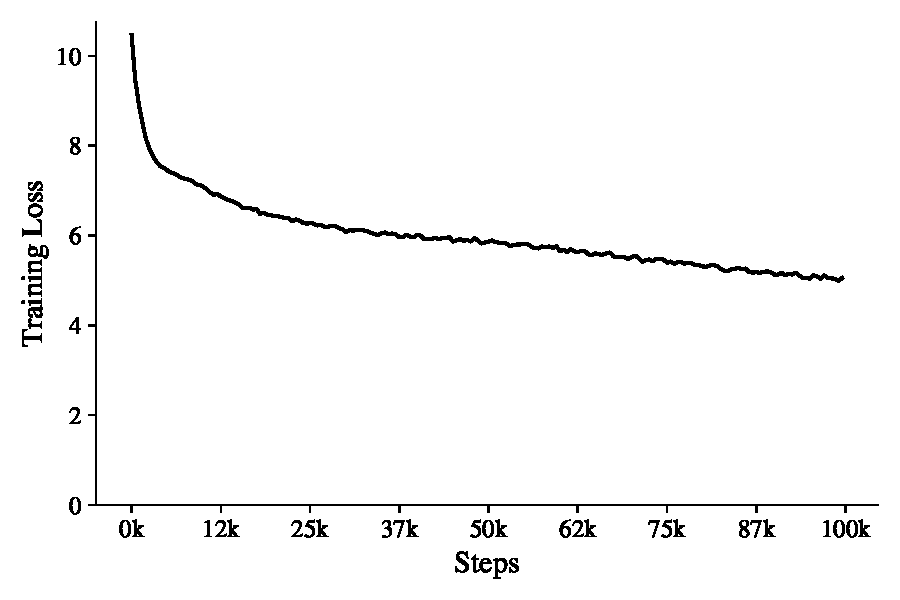
\includegraphics[width=0.5\textwidth]{figures/train_loss.pdf}
\caption{Training loss curve for the 126M-parameter model after 100k steps.}
\label{fig:training_curve}
\end{figure}

Using the pretraining corpora, we trained a model with 126M parameters, that will later on serve as bases for finetuning downstream tasks.
\libertus{} follows RoBERTa's pretraining architecture \cite{liu-etal-2019-roberta} and takes inspiration from \citet{conneau-etal-2020-unsupervised}'s work on scaling BERT models to multiple languages.

\subfile{tables/pretrain_hyperparams.tex}

Our hyperparameter choices closely resemble that of the original RoBERTa implementation as seen in Table \ref{table:pretrain_hyperparams}.
We also trained the same BPE tokenizer \citep{sennrich-etal-2016-neural} using the constructed corpora.
During model pretraining, we used the AdamW optimizer with $\beta_2$=0.98 and a weight decay of 0.01.
The base model underwent training for 100k steps with a learning rate of 2e-4.
We used a learning rate scheduler that linearly warms up during the first quarter of the training process, then linearly decays for the rest.
Figure \ref{fig:training_curve} shows the training curve.

\subsection{Model Finetuning}

For each language, we finetuned a multitask model using spaCy \cite{honnibal-etal-2020-spacy}. 
The final system consists of a parts-of-speech (POS) tagger, morphological analyzer, and lemmatizer.

\paragraph{Parts-of-speech (POS) tagger:}
We employed a standard classifier that predicts a vector of tag probabilities for each token.
Each POS tag is a unique class that we assign exclusively to a token.
We trained a model by taking the context-sensitive vectors from our pretrained embeddings, and passing it to a linear layer with a softmax activation.
The network is then optimized using a categorical cross-entropy loss.

\paragraph{Morphological analyzer:}
Similar to the POS tagger, we treat morphological annotation as a token classification task.
Instead of directly modeling each feature, we made every unique combination of morphological features as a class.
The limitation of this approach is that it can only predict combinations that were present in the training corpora.

\paragraph{Lemmatizer:} 
We trained a neural-based edit tree lemmatizer \cite{muller-etal-2015-joint} by first extracting an edit tree for each token-lemma pair.
Because this process can result to hundreds of edit trees, we treat the problem of picking the correct tree as a classification task.
Here, each unique tree serves as a class and we compute a probability distribution over all trees for a given token.
To obtain the most probable tree, we passed the context-sensitive embeddings from our pretrained model to a softmax layer and trained the network with a cross-entropy loss objective.

\section{Results and Discussion}

Table \ref{table:main_results} shows the test scores for the shared task.
\lj{Talk about how you ranked against other teams?}
In this section, we will outline our internal evaluations and benchmarking experiments.


\begin{figure*}[t]
\centering
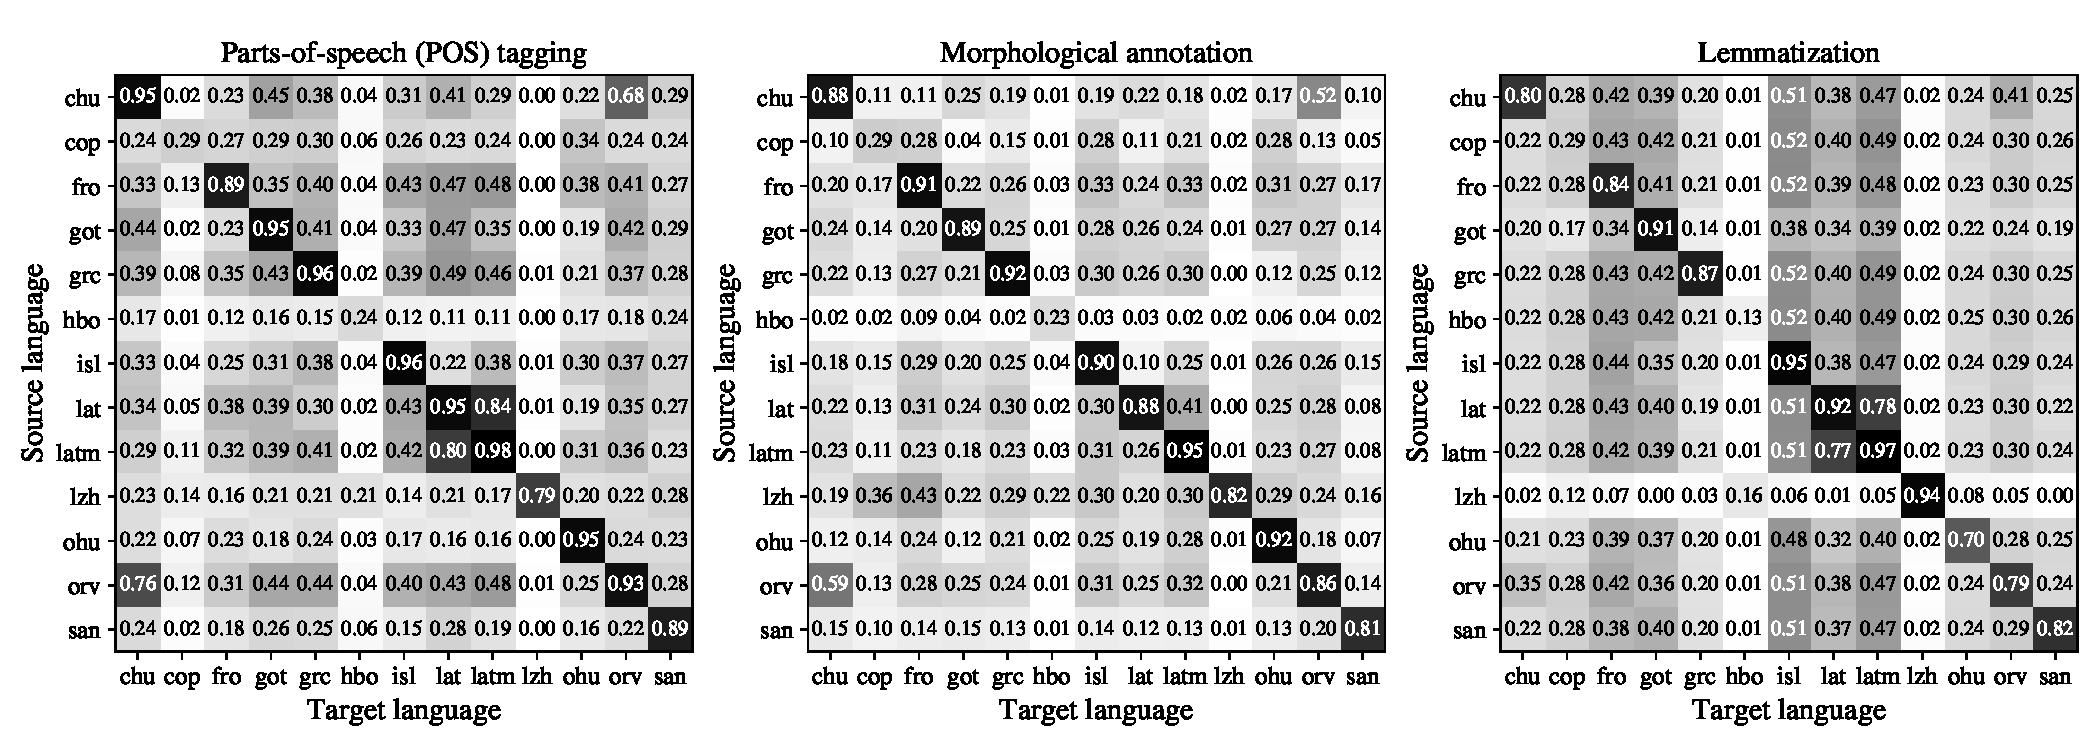
\includegraphics[width=\textwidth]{figures/cross_lingual.pdf}
\caption{Cross-lingual evaluation given a monolingual model from one language and a validation set in another.}
\label{fig:cross_lingual}
\end{figure*}


\subsection{Performance on the validation set}

First, we evaluated our finetuned models on the validation set.
Table \ref{table:validation_results} shows the results.

\subfile{tables/validation_results.tex}



\subsection{Evaluating cross-lingual capabilities}
\label{sec:results_crosslingual}

To test the cross-lingual capability of a language, we evaluated its finetuned model to the validation set of another.
Figure \ref{fig:cross_lingual} shows the results.

% it is possible to adapt a language on some tasks (e.g., morph annotation and lemmatization),
% some languages like lat, latm can also be used interchangeably in lemmatization




\section{Conclusion}

\section*{Limitations}

\paragraph{Use of BPE tokenizer:}

\paragraph{Pretrained LM size:}


\bibliography{custom}

\appendix

\section{Appendix}
\label{sec:appendix}

\subsection{Effect of different sampling strategies on pretraining performance}

We also explored different sampling strategies and their effect on the pretraining loss curve.
In our final system, we used the upsampling strategy as it provides clear benefit compared to others.

We examined the following configurations:
\begin{itemize}
  \item \textbf{None:} we used the original dataset without any data sampling or augmentation.
  \item \textbf{Upsampling:} we upsampled each language to ensure that the number of their unique tokens is greater than or equal to the most dominant language.
  \item \textbf{Averaging:} we took the average number of unique tokens in the whole set and up-/downsampled each language based on this value.
\end{itemize}

Figure \ref{fig:effect_sampling} shows that upsampling provides the clearest benefit for our pretrained model.

\subsection{Finetuning a model per language vs. monolithic system}

We also investigated if finetuning a model per language is more effective against a monolithic system, i.e., training on the full multilingual annotated corpora.
We found out that although more expensive, finetuning a model per language still yields the best results. 
Table \ref{table:full_vs_langspecific} illustrates these results.

\subsection{Reproducibility}

The pretrained models can be found in ... while the source code to replicate the experiments can be found on ...

\subsection{Alternative approach}

We also considered to use multi-hash embeddings \cite{miranda-etal-2022-multi} as an alternative approach.
Instead of pretraining, these embeddings use orthographic features (e.g., prefix, suffix, norm, shape) to create a word vector table.
This approach also applies the hashing trick, inspired by Bloom filters \cite{bloom-1970-space}, to decrease the vector table's memory footprint.

Figure \ref{fig:benchmarking} shows the results in comparison to our final system.
It is notable that simple orthographic features are competitive with our transformer-based model.
However, we chose to submit the transformer-based pipeline as our final system because it still outperforms the multi-hash embed method in the majority of our language-task pairs. 
We still recommend investigating this approach further because the hash-embed method has noticeable efficiency gains in terms of model size.

\end{document}
